\DeclareOldFontCommand{\bf}{\normalfont\bfseries}{\mathbf}
\documentclass[
	fontsize=12pt,
	paper=a4,
	bibliography=totoc,
	index=totoc,
	listof=totoc,
	footinclude=false,
	BCOR16mm,
	DIV=10
	]{scrbook}


%%%%% include settings
% Included by MAIN.TEX
% Defines the settings for the CAMP report document

% use german characters as well
\usepackage[utf8]{inputenc}       % allow UTF-8 characters
%\usepackage[ansinew]{inputenc}       % allow ANSII-new characters

\renewcommand{\sectfont}{\normalfont \bfseries}        % Schriftart der Kopfzeile

% manipulate footer
\usepackage{scrpage2}
\pagestyle{scrheadings}
\ifoot[\footertext]{\footertext} % \footertext set in INFO.TEX
%\setkomafont{pagehead}{\normalfont\rmfamily}
\setkomafont{pagenumber}{\normalfont\rmfamily}


%\usepackage{algorithm}
%\usepackage{algpseudocode}
%\floatname{algorithm}{Algorithmus}
%\usepackage{framed}
%\usepackage{multicol}

%% allow sophisticated control structures
\usepackage{ifthen}

% use Palatino as default font
\usepackage{palatino}

% enable special PostScript fonts
\usepackage{pifont}

%to use the subfigures
\usepackage{subfigure}

%\usepackage{wrapfig}
\usepackage{listings}
\usepackage{color}
\usepackage[svgnames]{xcolor}
\usepackage{colortbl}

% for js listings
\usepackage{caption}
\usepackage{jslistings}

\usepackage{url}
\usepackage{stackengine}

%\makeatletter 
%\g@addto@macro\UrlBreaks{ 
%  \do\a\do\b\do\c\do\d\do\e\do\f\do\g\do\h\do\i\do\j 
%  \do\k\do\l\do\m\do\n\do\o\do\p\do\q\do\r\do\s\do\t 
%  \do\u\do\v\do\w\do\x\do\y\do\z\do\&\do\1\do\2\do\3 
%  \do\4\do\5\do\6\do\7\do\8\do\9\do\0} 
%% \def\do@url@hyp{\do\-} 
%\makeatother 

\usepackage{url}
\urlstyle{same}

%% show program code\ldots
%\usepackage{verbatim}
%\usepackage{program}

%% enable TUM symbols on title page
\usepackage{styles/tumlogo}


\usepackage{multirow}

%% use colors
\usepackage{color}

%% make fancy math
\usepackage{amsmath}
\usepackage{amsfonts}
\usepackage{amssymb}
\usepackage{textcomp}
\usepackage{yhmath} % f�r die adots 
%% mark text as preliminary
%\usepackage[draft,german,scrtime]{prelim2e}

%% create an index
\usepackage{makeidx}

% for the program environment
%\usepackage{float}
\usepackage{tocbasic}

%% load german babel package for german abstract
%\usepackage[german,american]{babel}
\usepackage[ngerman]{babel}
%\selectlanguage{german}

% use initals dropped caps - doesn't work with PDF
%\usepackage{dropping}


\usepackage{styles/shortoverview}
%----------------------------------------------------
%      Graphics and Hyperlinks
%----------------------------------------------------


%% check for pdfTeX
\ifx\pdftexversion\undefined
 %% use PostScript graphics
 \usepackage[dvips]{graphicx}
 \DeclareGraphicsExtensions{.eps,.epsi}
 \graphicspath{{figures/}{figures/review}} 
 %% allow rotations
 \usepackage{rotating}
 %% mark pages as draft copies
 %\usepackage[english,all,light]{draftcopy}
 %% use hypertex version of hyperref
 \usepackage[hypertex,hyperindex=false,colorlinks=false,breaklinks]{hyperref} 
 %% breaks urls if they are too long
 \usepackage{breakurl}
\else %% reduce output size \pdfcompresslevel=9
 %% declare pdfinfo
 %\pdfinfo { 
 %  /Title (my title) 
 %  /Creator (pdfLaTeX) 
 %  /\dfrac{Author}{den} (my name) 
 %  /Subject (my subject	) 
 %  /Keywords (my keywords)
 %}
 %% use pdf or jpg graphics
 \usepackage[pdftex]{graphicx}
 \DeclareGraphicsExtensions{.jpg,.JPG,.png,.pdf,.eps}
 \graphicspath{{figures/}} 
 
 %% allow rotations
 \usepackage{rotating}
 %% use pdftex version of hyperref
 \usepackage[pdftex,colorlinks=true,linkcolor=black,citecolor=black,%
 anchorcolor=black,urlcolor=black,bookmarks=true,%
 bookmarksopen=true,bookmarksopenlevel=0,plainpages=false,%
 bookmarksnumbered=true,hyperindex=false,pdfstartview=%
 ]{hyperref}
%
%\usepackage[pdftex,colorlinks=false,linkcolor=red,citecolor=red,%
% anchorcolor=red,urlcolor=red,bookmarks=true,%
% bookmarksopen=true,bookmarksopenlevel=0,plainpages=false%
% bookmarksnumbered=true,hyperindex=false,pdfstartview=%
% ]{hyperref}




%% Fancy chapters
%\usepackage[Lenny]{fncychap}
%\usepackage[Glenn]{fncychap}
%\usepackage[Bjarne]{fncychap}

%\usepackage[avantgarde]{quotchap}

% set the bibliography style
\bibliographystyle{unsrtnat}

\usepackage{textcomp}
%\definecolor{listinggray}{gray}{0.9}
%\definecolor{lbcolor}{rgb}{0.9,0.9,0.9}
%\lstset{language=XML}

\usepackage[all]{hypcap}
\pdfminorversion=6

\usepackage[T1]{fontenc}
\usepackage{epsfig}
\usepackage[numbers,sort&compress]{natbib}
\usepackage{bm}
\usepackage[normalem]{ulem}

%% Do tabs
\usepackage{tabto}

\addtokomafont{captionlabel}{\bfseries}

%% Use enumeration of subsubsections
\setcounter{secnumdepth}{3}

%% Use footnote numbering for whole document
\usepackage{chngcntr} 
\counterwithout{footnote}{chapter}

\DeclareNewTOC[
    counterwithin=chapter,
    float, type=codelisting, types=codelistings,
    name={Listing}, listname={List of Code}
]{loc}
\setuptoc{loc}{chapteratlist}

%% \DeclareNewTOC[%
%	counterwithin=chapter,%
%	hang=2em,%
%	type=example,%
%	types=examples,%
%	nonfloat,%
%	name=Beispiel,%
%	listname={Beispielverzeichnis}%
%]{loex}
%\setuptoc{loex}{chapteratlist}

%\DeclareNewTOC[%
%	counterwithin=chapter,%
%	hang=2em,%
%	type=definition,%
%	types=definitions,%
%	nonfloat,%
%	name=Begriff,%
%	listname={Begriffsverzeichnis}%
%]{lode}
%\setuptoc{lode}{chapteratlist}

%\setlength{\textfloatsep}{-20pt}
%\setlength{\belowcaptionskip}{10pt plus 0pt minus 0pt}

%%%%% include command
% Commands to be used within the TUM report document
% Included by MAIN.TEX
% Please include your own cool commands here. 
% Be only sure to comment it sufficiently so others can use it.

%-------------------------------------------------------------
%                      Own Commands
%-------------------------------------------------------------


%-------------------------------------------------------------
% math stuff -------------------------------------------------

% nice R, N, C
\newcommand{\nat}{\mathbb{N}}
\newcommand{\real}{\mathbb{R}}
\newcommand{\compl}{\mathbb{C}}



% norm
\newcommand{\norm}[1]{\left\| #1 \right\|}

% un demi
\newcommand{\half}{\frac{1}{2}}

% parantheses
\newcommand{\parenth}[1]{ \left( #1 \right) }
\newcommand{\bracket}[1]{ \left[ #1 \right] }
\newcommand{\accolade}[1]{ \left\{ #1 \right\} }
%\newcommand{\angle}[1]{ \left\langle  #1 \right\rangle }

% partial derivative: %#1 function, #2 which variable
% simple / single line version
\newcommand{\pardevS}[2]{ \delta_{#1} f(#2) }
% fraction version
\newcommand{\pardevF}[2]{ \frac{\partial #1}{\partial #2} }

% render vectors: 3 and 4 dimensional
\newcommand{\veciii}[3]{\left[ \begin{array}[h]{c} #1 \\ #2 \\ #3	\end{array} \right]}
\newcommand{\veciv}[4]{\left[ \begin{array}[h]{c} #1 \\ #2 \\ #3 \\ #4	\end{array} \right]}

% render matrices: 3  dimensional (arguments in row first order)
\newcommand{\matiii}[9]{\left[ \begin{array}[h]{ccc} #1 & #2 & #3 \\ #4 & #5 & #6 \\ #7 & #8 & #9	\end{array} \right]}
%DOESN'T WORK,DON'T KNOW WHY \newcommand{\mativ}[16]{\left[ \begin{array}[h]{cccc} #1 & #2 & #3 & #4 \\ #5 & #6 & #7 & #8 \\ #9 & #10 & #11 & #12 \\ #13 & #14 & #15 & #16 \end{array} \right]}


%-------------------------------------------------------------
%-------------------------------------------------------------


%-------------------------------------------------------------
% some abreviations ------------------------------------------
\newcommand{\Reg}{$^{\textregistered}$}
\newcommand{\reg}{$^{\textregistered}$ }
\newcommand{\Tm}{\texttrademark}
\newcommand{\tm}{\texttrademark~}
\newcommand {\bsl} {$\backslash$}

%-------------------------------------------------------------
%-------------------------------------------------------------



%-------------------------------------------------------------
% formating --------------------------------------------------

% Theorem & Co environments and counters
%\newtheorem{theorem}{Theorem}
%\newtheorem{lemma}[theorem]{Lemma}
%\newtheorem{corollary}[theorem]{Corollary}
%\newtheorem{remark}[theorem]{Remark}
%\newtheorem{definition}[theorem]{Definition}
%\newtheorem{equat}[theorem]{Equation}
%\newtheorem{example}[theorem]{Example}
% \newtheorem{algorithm}[theorem]{Algorithm}

% inserting figures
%\newcommand{\insertfigure}[4]{ % Filename, Caption, Label, Width percent of textwidth
%	\begin{figure}[htbp]
%		\begin{center}
%			\includegraphics[width=#4\textwidth]{#1}
%		\end{center}
%		\vspace{-0.4cm}
%		\caption{#2}
%		\label{#3}
%	\end{figure}
%}

%-------------------------------------------------------------
%-------------------------------------------------------------


% new stuff (Michael)

%-------------------------------------------------------------
%-------------------------------------------------------------

\newcommand{\insertfigure}[3]{ %filename and label, width, caption
	\begin{figure}
		\center
		\includegraphics[width=#2\columnwidth]{images/#1}
		\vspace{-0.2cm}
		\caption{#3}
		\label{fig:#1}
	\end{figure}
}

\newcommand{\insertdefinition}[3] { %label, caption, text
%	\begin{definition-}
		\KOMAoptions{captions=nooneline}
		\captionof{definition}[#2]{\textbf{#2}: #3}
		\label{def:#1}
		\vspace{0.2cm}
		\KOMAoptions{captions=oneline}
%	\end{definition-}
}

\newcommand{\insertexample}[3] { %label, caption, text
	\begin{example-}
		\KOMAoptions{captions=nooneline}
		\captionof{example}[#2]{\textbf{#2}:}
		\label{ex:#1}
		\KOMAoptions{captions=oneline}
		\setlength\parindent{1em}
		#3
	\end{example-}
}

\newcommand{\insertlst}{
	\lstset{
		basicstyle=\small,
		keywordstyle=\bfseries,
		commentstyle=\color{green!50!black!100}, 
		stringstyle=\ttfamily, 
		language=Java,                % choose the language of the code
		frame=single,	                % adds a frame around the code
		aboveskip=11pt,
		belowskip=11pt,
		breaklines=true,                % sets automatic line breaking
		breakatwhitespace=false,  % sets if automatic breaks should only happen at
		showspaces=false,
		showstringspaces=false
	}
}



% Set here the title, authors and other stuff to be used for the cover
% This file is used by MAIN.TEX



% set title, authors and stuff for the cover
\def\doctype{Master Thesis}
\def\title{Offline caching in web applications for AntidoteDB} 
\def\author{Server Khalilov}
\def\date{DD. April 2018}

% text to appear in the footer
\def\footertext{}


%%%%% global hyphenation
\hyphenation{
}

\sloppy

\makeglossary

\begin{document}
\renewcommand{\chaptername}{Chapter}
\renewcommand\contentsname{Contents}
\renewcommand{\tablename}{Table}
\renewcommand{\listtablename}{List of Tables}
\renewcommand{\figurename}{Figure}
\renewcommand{\listfigurename}{List of Figures}
\renewcommand{\bibname}{Bibliography}
\renewcommand{\appendixname}{Appendix}

	%%%%% Deckblatt
	\frontmatter	
	% The front cover for the TUM report document.
% Included by MAIN.TEX


%--------------------------------------------------
% The Front Cover
%--------------------------------------------------

% The front cover for the TUM document.
% Included by MAIN.TEX


%--------------------------------------------------
% The Front Cover
%--------------------------------------------------

% correct BCOR - undo at the end !!!
\def\bcorcor{0.15cm}
\addtolength{\hoffset}{\bcorcor}

\thispagestyle{empty}

 \vspace{4cm}
\begin{center}
	     %  \oTUM{4cm}
	   
	   \vspace{5mm}     
	   \large Department of Computer Science\\ 
	   \vspace{0.5cm}
	 \large University of Kaiserslautern\\
    \vspace{1mm}
        
	\end{center}
		

\vspace{20mm}
\begin{center}

   {\LARGE \doctype}

  \vspace{15mm}  
  {\huge\textbf \title\par}%[3ex]
  
  
  \vspace{20mm}
   
  {\LARGE  \author}
  
  \vspace{10mm}
	
%	xxx@cs.uni-kl.de\\
	University of Kaiserslautern\\
	Department of Computer Science\\
	Software Engineering\\
	\ \\
	Leader:\\
	Prof. Dr. Arnd Poetzsch-Heffter\\
	\ \\
	Supervisor:\\
	Dr. rer. nat. Annette Bieniusa\\
  
%  \includegraphics[width=8cm]{images/Marimba}
  
  \vspace{10mm}
  
  
\includegraphics[width=4cm]{styles/tulogo}
  
  \end{center}
	
	%%%%% Abstract und Disclaimer
	\cleardoubleoddemptypage
	\thispagestyle{plain}
	% German abstract for the CAMP report document
% Included by MAIN.TEX

\begin{center}
{\Large \textbf Zusammenfassung}
\end{center}
\vspace{1cm}

Zusammenfassung auf deutsch
	\cleardoubleoddplainpage
	% Abstract for the TUM report document
% Included by MAIN.TEX

\begin{center}
{\Large \textbf Abstract}
\end{center}
\vspace{1cm}


The goal of this thesis is to design a web-client for Antidote-DB with a support of caching with a further implementation. In order to achieve this goal, the understanding of how CRDT works needs to be reached. The paper could be logically divided into two parts: firstly, the problem of designing mentioned solution is going to be discussed. Secondly, there is an implementation part and description how specific problems were tackled.
	
	\cleardoubleevenplainpage
	%\selectlanguage{german}
	\vspace*{0.72\textheight}
	\noindent
Ich versichere hiermit, dass ich die vorliegende Masterarbeit mit dem Thema
"`\title"' selbstständig verfasst und keine anderen als die angegebenen Hilfsmittel benutzt habe. \\
Die Stellen, die anderen Werken dem Wortlaut oder dem Sinn nach entnommen wurden, habe ich durch die Angabe der Quelle kenntlich gemacht.
	
	\vspace{8mm}
	\noindent
	Kaiserslautern, den \date \hspace{3,5cm} \author
%\selectlanguage{english}
\newpage
	
	%%%%% Inhaltsverzeichnis
	\cleardoubleoddplainpage
	\pdfbookmark[1]{Contents}{toc}
	\tableofcontents
	
	%%%%% Alle anderen Kapitel, Anhang und Verzeichnisse
	\mainmatter
	
		\cleardoubleoddplainpage
		\label{part:Introduction}
		\chapter{Introduction}
\label{Introduction}

In this chapter we are going to discuss the motivation, research questions and the scope of this thesis.

o Problem context (What is the broader context of this work?) 
o Problem description (What is the specific problem or challenge addressed by this work?) 
o Research question(s) (What are the actual questions that should be answered by this research? Why are they interesting? To whom? Why is there no obvious answer? If this is getting too much, then details of discussion can be deferred until later, e.g., to the methodology section.) 
o Summary of results and contributions (What is the outcome of this work in simple terms?) 
o Structure of the thesis (Introduce briefly the remaining chapters.)

\section{Motivation}

The motivation of this thesis is to explore the possibilities of implementing a web-client with a cache on a client-side. 

\section{Research questions}

The following research questions are going to be addressed in this thesis:
\\\\
\textbf{RQ1.} How efficient is it to use a web-client with cache rather than without it?
\\\\
\textbf{RQ2.} What are the methods available to implement web-applications that would be able to work off-line and in the conditions of poor network connections?
\\\\
\textbf{RQ3.} What could be a scalable solution for transmitting CRDT data between a server and clients?

		\cleardoubleoddplainpage
		\label{part:Background}
		\chapter{Theoretical background}
\label{Background}

In this chapter, we are going to introduce the reader to the theoretical concepts, which represent a prerequisite to have an understanding of this thesis.

\section{Main concepts}
\label{Background-Main}

\textit{Distributed database} is ``a collection of multiple, logically interrelated databases distributed over a computer network''\cite{11}. A \textit{geo-distributed database}, in its turn, is a database, which is spread across two or more geographically distinct locations and runs without experiencing performance delays. The maintaining of such databases brings its challenges. As the database is spread across several locations, there should be a replication process in order to ensure that replicas of that database synchronise and have the latest state of the data. This replication process should be fast, because if there are two replicas of the database, then whenever there is some information written to the first replica, it should be accessible to users, who use the second one. That is the problem of the availability, but before the information at replicas becomes available, it first should be checked over the consistency, as the states of the replicas should be equal. That is a complex task to solve. 

Working with such a distributed database, whenever the data is needed to be read or changed in any way, a transaction should be started, executed and closed. A \textit{transaction} is a basic unit of computing, which consists of a sequence of operations that are applied atomically on a database. Transactions transform a consistent database state to another consistent database state. A transaction is considered to be \textit{correct} if it obeys the rules, specified on the database. As long as each transaction is correct, a database guarantees that concurrent execution of user transactions will not violate database consistency \cite{11}. \textit{Consistency} requires transactions to change the data only according to the specified rules. An example of consistency rule can be the following: let us say that in a bank database the bank account number should only consist of integer numbers. If an employee tries to create an account that contains something other than integer numbers in it, then the database consistency rule will disallow it. Consistency rules are important as they control the incoming data and reject the information, which does not fit.

\textit{Sequential consistency} and \textit{linearizability} are two consistency conditions that are well-known. Sequential consistency requires that all of the data operations appear to have executed atomically (i.e. independently), in some sequential order. When this order must also preserve the global ordering of non-overlapping operations, this consistency is called linearizability\cite{27}. Linearizability guarantees that the same operations are applied in the same order to every replica of the data item\cite{12}. Serializability is a guarantee about transactions, that they are executed serially (i.e. without overlapping in time) on every set of the data items\cite{12}. Serializability is more strict than sequential consistency, as the granularity of sequential consistency is a single operation, while for serializability it is a transaction. As a result, when serializability is satisfied, the sequential consistency is also satisfied, but not vice versa.

Now, let us introduce different consistency models and the one we will follow in the designing part of WebCure. 

As stated by \citet{10}, ``\textit{strong consistency} model could be described in the following way: whenever the update is performed, everyone knows about it''. It means that there is a total order of updates, and reads are guaranteed to return the latest data, regardless of which replica is the source of the response. The advantage of strong consistency is that the database is always in a consistent state and to disadvantages, we can add low latency, as there is a delay for making sure that all the replicas are in a consistent state before any other read / write requests could be processed. The latency point is a huge drawback for the performance, especially if a strong consistency model is considered to be used as a solution for the web, where users usually expect high responsiveness and availability. 

The main point of replicating data is to improve such aspects as reliability, availability, performance and latency. However, according to CAP Theorem\cite{29}, a distributed database can only have two of the three properties: consistency, availability and partition tolerance. This theorem is fundamental, as it makes people think towards the trade-off between those three properties for a specific use case. There are some weaker consistency models, where the results of requests can alter depending on the replica\cite{28}.  In this thesis, we will stick with partial \textit{causal consistency}. As it is stated in \citet{7}, causal consistency is ``the strongest available and convergent model''. They continue their statement saying that ``under causal consistency, every process observes a monotonically non-decreasing set of updates that includes its updates, in an order that respects the causality between operations''. As the causal ordering is respected, it makes it easier for programmers to reason, as it gives the guarantee that related events are visible in the order of occurrence, while the events, which have no relation to each other, can be in a different order in different replicas. Let us consider an example of an application for some of social networks. There, a reply to a wall post happens after the original post is published. Thus, users should not see the reply before the original post is observable. This type of guarantees is provided by causal consistency. Looking at \figref*{fig:theory3} we can see that on the left subfigure, the user can see the original wall post as well as the reply, while on the right subfigure, without causal consistency, the user sees only the reply, while the original wall post is missing. 

\begin{figure}%
    \centering
    \def\svgwidth{0.4\linewidth}
    \subfloat[]{{\input{images/causal/causal_true.pdf_tex}}}%
    \qquad
    \def\svgwidth{0.4\linewidth}
    \subfloat[]{{\input{images/causal/causal_false.pdf_tex}}}%
    \caption{An example of how a causally consistent behaviour (a) and the one that is not (b) could work in a social network.}%
    \label{fig:theory3}%
\end{figure}





\section{AntidoteDB}
\label{2-antidotedb}

For this thesis, one of the core parts of the architecture of WebCure belongs to the database called AntidoteDB\cite{4}. It helps programmers to write correct applications and has the same performance and horizontal scalability as AP / NoSQL\cite{14}, while it also:

\begin{itemize}
\item {is geo-distributed, which means that the datacenters of AntidoteDB could be spread across anywhere in the world;}
\item {groups operations into atomic transactions\cite{9, 15};}
\item {delivers updates in a causal order and merges concurrent operations.}
\end{itemize} 

Merging concurrent operations is possible because of CRDTs\cite{2}, which are used in AntidoteDB. It supports counters, sets, maps, multi-value registers and other types of data that are designed to work correctly in the presence of concurrent updates and failures. The usage of CRDTs allows the programmer to avoid problems that are common for other databases like NoSQL, which are fast and available, but hard to program against\cite{15}. We will cover the topic of CRDTs later in this chapter.

Apart from that, to replicate the data AntidoteDB implements the \textit{Cure}\cite{15} protocol. It is a highly scalable protocol, which provides causal consistency. 

To ensure the guarantees it offers, AntidoteDB uses timestamps, indicating the time after the transaction. Timestamps are considered to be unique, totally ordered, and consistent with causal order, which means that if \textit{operation 1} happened before \textit{operation 2}, then the timestamp related to the \textit{operation 2} is greater than the one related to the \textit{operation 1}\cite{2}.Whenever the update operation has to be applied, it is also possible to provide a minimum time from what that update should be performed. This information is useful when a client is working with a server, which is based on AntidoteDB. In such cases, when one data centre stops working, the client can reconnect to another one. As a client can remember the latest timestamp for the data it has worked on, the failover to another data centre is possible without any additional efforts, as the timestamp information will help the client to request only the data, which have timestamps greater than the one, which is already stored at the client.

\section{CRDTs}
\label{2-crdts}

As it is stated in the work of \citet{3}, a CRDT is an abstract datatype, which is designed for a possibility to be replicated at multiple processes and possesses the following properties:


    \begin{itemize}
        \item {The data at any replica can be modified independently of other replicas;}
        \item {Replicas deterministically converge to the same state when they received the same updates.}
    \end{itemize}

Replication is a fundamental concept of distributed systems, well studied by the distributed algorithms community\cite{2}. There are two models of replication that are considered: state-based and operation-based. We are going to introduce our reader to both of them below. 

\subsection*{Operation-based replication approach}

\begin{figure}[!htb]
    \begin{center}
    \def\svgwidth{\linewidth}
    \input{images/crdts-replication/op-based.pdf_tex}
    \caption {Operation-based approach\cite{2}. <<S>> stands for source replicas and <<D>> for downstream replicas. }
    \label{fig:theory1}
\end{center}
\end{figure}

In this thesis, we are going to use the operation-based replication approach, where replicas converge by propagating operations to every other replica\cite{3}. Once an operation is received in a replica, it is applied locally. Afterwards, all replicas would possess all of the updates. In \figref*{fig:theory1}, we can see that firstly operations \textit{f(x\textsubscript{i})}, \textit{g(x\textsubscript{i})} applied locally at source replicas \textit{x\textsubscript{i}}, and then the operations are conveyed to all the other replicas. The second part of this process is named \textit{downstream} execution.

This replication approach infers that replicas do not exchange full states with each other, which is a positive concerning efficiency. Not always, though, as it depends on the task. Sometimes, applying multiple operations at every replica could be costly, and this is where state-based replication approach is beneficial.

% TODO What are the requirements for the op-based CRDTs to work correctly?
% Give an example of an op-based CRDT specification? counter!!!

\subsection*{State-based replication approach}
\begin{figure}[!htb]
    \begin{center}
    \def\svgwidth{\linewidth}
    \input{images/crdts-replication/state-based.pdf_tex}
    \caption {State-based approach\cite{2}. <<S>> stands for source replicas and <<M>> for merging stages.}
    \label{fig:theory2}
\end{center}
\end{figure}

The idea of this approach is kind of opposite to the operation-based one. Here, every replica, when it receives an update, first applies it locally. Afterwards, it sends its updated state to other replicas. Following this way, every replica sends its current full state to other replicas. Afterwards, the merge function is applied between a local state and a received state, and every update eventually is going to appear at every other replica in the system. We can see this it in the \figref*{fig:theory2}, where \textit{x\textsubscript{i}} stands for replicas, \textit{f(x\textsubscript{i})}, \textit{g(x\textsubscript{i})} stands for the functions that apply updates locally at source replicas before sending a new full state for a follow-up merges to other replicas in the system.

%What are the requirements for the state-based CRDTs to work correctly?

There are different types of CRDTs, yet, we will consider three of them: counters, sets and multi-value registers. We will give a brief description to each of the mentioned datatypes below.

\subsection*{Counter}

Counter is a datatype, which keeps track on its state, which is an integer number. The value of the Counter could be modified by the operations \textit{inc} and \textit{dec} that increases or decreases the state by one unit, accordingly\cite{3}. The concurrency semantics for this datatype is that a final state of the object reflects all the performed operations on it. In other words, to calculate the state of the Counter, it is needed to count the number of increments and subtract the number of decrements. 

\subsection*{Add-wins Set}

Add-wins Set\footnote{For the simplicity of reading, later it goes as Set.} datatype represents a collection of objects with a specific handling of concurrent updates performed over them. In case of concurrent updates on the same object, \textit{add} operations in Set win against \textit{remove} operations. If, for example, there is an empty set \textit{} and two concurrent operations applied to it -- \textit{add a} and \textit{remove a}, then the result is going to be \textit{\{a\}}, as \textit{add} operation wins. A \textit{remove} operation will ``overwrite'' an \textit{add} operation only when it happens after it\cite{3}. 

\subsection*{Multi-value Register}

This datatype maintains a value and provides a \textit{write} operation of updating that value. The exciting part about multi-value Registers is their concurrency semantics. In the case of two or more updates happening at the same time, all values are kept. Thus, the state of the register will consist of all the concurrently written updates for further processing. However, any additional single \textit{write} operation will overwrite the previous state of the register, even if it consisted of multiple values\cite{39}.
		
		\cleardoubleoddplainpage
		\label{part:Problem Analysis}
		\chapter{Problem Analysis}
\label{Problem Analysis}

Might be not needed

\section{Requirements}

This chapter is needed specifically, if the work is meant to design or implement some sort of software system. In good alignment with basic software engineering practice, the requirements for this system have to be developed systematically. Each requirement should have a short name, a short description, and some illustration. Additional elements are priorities (must, should, can), pointers to related work, and a discussion of the challenges involved.

		\cleardoubleoddplainpage
		\label{part:Design}
		\chapter{Design}
\label{Design}

Design or Approach

\section{Modern offline applications}
		
		\cleardoubleoddplainpage
		\label{part:Technologies}
		\chapter{Technologies}
\label{Technologies}

This chapter consists of detailed description of used technologies to accomplish thesis goal.

\section{Service Workers}
\section{IndexDB database}
		
		\cleardoubleoddplainpage
		\label{part:Architecture}
		\chapter{Architecture}
\label{Architecture}

Architecture
\section{General overview of the architecture}
\section{Communication protocol description}

		\cleardoubleoddplainpage
		\label{part:Implementation}
		\chapter{Implementation}
\label{Implementation}

In this chapter, we are going to explain the major problems that we encountered during the implementation phase.

Addressing the client, we will name the frameworks and techniques that we are going to use in the implementation phase. Concerning the server, which is going to provide the RESTful interface, though, we will cover the use cases.

\begin{figure}[!htb]
    \begin{center}
    \setlength{\fboxsep}{4pt}%
    \setlength{\fboxrule}{1pt}%
    \stackunder{\fbox{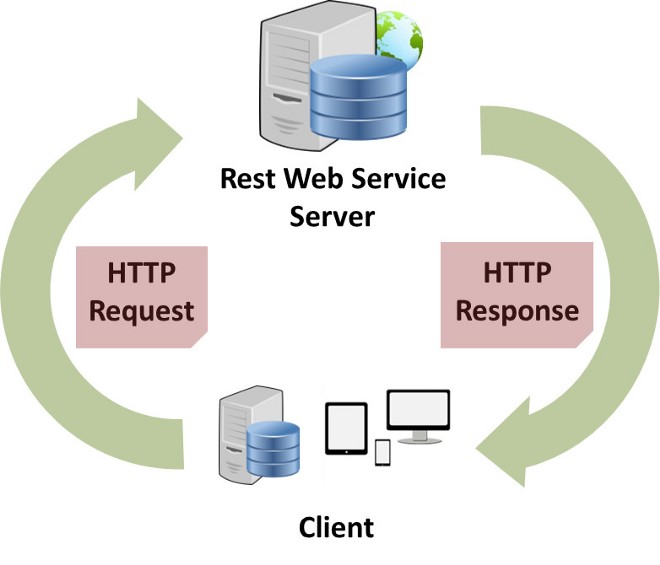
\includegraphics[width=0.5\linewidth]{images/design/clientserver.jpeg}}}%
    {\scriptsize%
     Source: \url{https://cdn-images-1.medium.com/max/660/1*EbBD6IXvf3o-YegUvRB_IA.jpeg}}
    \caption {A look at the server-client architecture with a RESTful interface.}
    \label{fig:design1}
\end{center}
\end{figure}


		\cleardoubleoddplainpage
		\label{part:Evaluation}
		\chapter{Evaluation}
\label{Evaluation}

Evaluation

This chapter is needed, when results from the previous chapters need to be systematically discussed. This is the case, when an implementation needs to be assessed, or the results of a case study or an experiment need to be interpreted.


- add the comparison between your approach and the other, in related work.

- add the test coverage statistics




		\cleardoubleoddplainpage
		\label{part:Conclusion}
		\chapter{Conclusion}
\label{Conclusion}

In this chapter, we will make a summary of our work and suggest some possibilities for future work.

\section{Summary}
\label{summary}

The work of this thesis mostly concentrated on designing such a client-server system, which would let replicating the data on a client machine. That would allow the user for offline operation at times, when there is no internet connection available, or when it is poor. Moreover, there are requirements for the system such as the possibility to maintain the data at client side as well, and synchronise it with a cloud storage server, when the mode of the client switches from offline to online. Additionally, after the system was designed, it was needed to be implemented, and its feasibility and performance should have been evaluated.

This task was achieved in a framework, which we named WebCure. Firstly, we designed a stable protocol for the communication between a client and a server. Then, we made a research on available technologies, which would allow us to implement the system in a way it is intended to work. Next, we developed a presentation application, which demonstrates the work of WebCure on an example of a set CRDT. After this step, we took a calendar application, which was already built based on AntidoteDB, and extended it to work with WebCure in order to evaluate the outcome. It turned out that, as expected, that the extended version of the calendar has a much shorter response time, better availability, while still keeping its original functionality and letting its users work both offline and online. 

\section{Future Work}
\label{futurework}

Different circumstances create uncertainty with the current design of the application. In this section, we would like to discuss these situations, while keeping the answers to them open for future improvements.

\section*{Missing acknowledgement}

In the current design of the WebCure, when a client is online and makes a request to the server with an update, the server sends back the acknowledgement, so the client knows that the requested operation was applied on the server side. However, there is a topic for discussion in this use case. Imagine that the server does not send back the acknowledgement. There are two possibilities:

\begin{itemize}
    \item {The update was applied on the server, but the connection failed when the acknowledgement was about to be sent back to the client;}
    \item {The update was not applied on the server, and the client did not receive the acknowledgement because of that.}
\end{itemize}

However, the problem is that a client does not know, which of the above situations happened. 

One of the solutions could be the following: it does not matter, whether the update was applied on the server or not. A client will send the update again, while it has not received an acknowledgement, regardless of what happens on the server's side. Nevertheless, in this case, updates must be uniquely identifiable, in order not to apply on the server the same update twice.

The other possibility is to have a double verification on the server side. For example, a client sends an update to the server. After that, the server should send a message back that it received an update. Next, if a client received that message with acknowledgement, it sends another message to the server that it is possible to apply the update. 

Though, the above information represents our thoughts on the problem, which is not necessarily a solution to it.  

\section*{Automatic updates of data at a client}

The current design of WebCure requires that after a client sends a request with an update to the server and receives an acknowledgement, it should then still send another read request in order to update the data on its side. However, this behaviour can be improved. For example, in some cases, it might be needed that a client acquires updates from the server automatically. To extend WebCure with such functionality, our suggestion would be to use Push Notifications feature\cite{32} of a service worker. The service worker can receive push messages from a server, even when the application is not active. It shows notifications to the user on their device even when the application is closed and still notify about the updates of the data on the server side.

\subsection*{Consistency guarantees}

\begin{figure}[!htb]
    \begin{center}
    \def\svgwidth{\linewidth}
    \input{images/architecture/future.pdf_tex}
    \caption {The case of breaking causal consistency guarantees in the current protocol.}
    \label{fig:final}
\end{center}
\end{figure}

In the current protocol design, there is a possibility to break the causality of applied operations, and that is what we would like to consider. There is a case with potential problems, which is illustrated in \figref*{fig:final}. There, a client reads the data by \textit{id} from the server, which has a \textit{value} associated with that \textit{id}, at the timestamp \textit{t\textsubscript{1}}. Once the client gets this data, it goes offline, performs some changes locally, and now it has the \textit{value'} associated with \textit{id}. Then, the connection gets back, and this update is sent to the server and applied. However, at this point, the connection breaks again, so the acknowledgement response from the server did not reach the client. That means, that at server side the update was applied and the element \textit{id} got its value changed to \textit{value'} at the timestamp \textit{t\textsubscript{2}}. Nevertheless, the client did not receive that information, the element \textit{id} at the client side still has local changes applied to it, which change its value to \textit{value'}. However, the interesting point here is that a client still has the timestamp \textit{t\textsubscript{1}}, stored on its side. Therefore, any further local updates performed at the client, once the internet connection is back again, will be sent to the server with information to apply them at the timestamp \textit{t\textsubscript{1}} and not \textit{t\textsubscript{2}}, how ideally it should be. The bad part here is that while our specific client is offline, some other clients could be communicating with the server at this time which means that the server could have received some updates from them as well. The current design of the protocol does not guarantee causal consistency in such situations. 

Discussing possible solutions, it all depends on the use case. Sometimes, freezing the client side functionality until it receives the acknowledgement from the server, might be acceptable. However, as it might take a long time, this is not a desirable solution. The other option is to check the states that are received after the server eventually responds (consisting of possible changes of the other clients) and find a solution by looking at the difference with the previous state, which is stored at the client side. However, this is a question, which is open for further investigation.
		
		\listoffigures
		\listoftables
		%\listoftoc{loex}
		%\listoftoc{lode}

		\cleardoubleoddplainpage
		\bibliography{bibliography/references}

\end{document}